



% \vspace{-2mm}
% \subsubsection{Memory Effects Across Frameworks}
% \label{subsec:memoryagentbench}

% \input{tables/Experiements - Memory}

% We evaluate memory behavior using MemoryAgentBench under a standardized protocol. All frameworks are accessed through a common interface (Section~\ref{subsec:bench_memory}) with identical chunking, ingestion order, and metrics, and all experiments use the same backend model (\texttt{gpt-oss-20b} on Groq\footnote{Although \texttt{gpt-oss-20b} supports context windows of up to 130K tokens, large accumulated contexts exceed tokens-per-minute limits (e.g., 250K TPM). While inserting delays between requests can mitigate this issue, large contexts require impractically long waiting times, making extreme accumulation infeasible for evaluation.}) without framework-specific tuning. Observed differences therefore reflect native memory architectures. We identify three paradigms: \emph{retrieval-centric} memory with persistent semantic storage and query-conditioned access, \emph{accumulation-based} memory that replays recent interactions directly into the prompt, and \emph{hybrid} memory combining long-term retrieval with bounded short-term accumulation. CrewAI follows a retrieval-centric design, Agno and the OpenAI SDK are accumulation-based, and LangGraph implements a hybrid architecture. LangGraph is evaluated in retrieval-only and hybrid modes across multiple context budgets, while the OpenAI SDK is tested under varying context windows to characterize pure accumulation scaling. Concordia and OpenAgents are excluded: Concordia targets generative narrative simulation rather than task-oriented memory, and OpenAgents lacks a native memory abstraction, delegating it entirely to user-defined components and preventing fair comparison.



% Table~\ref{tab:memorybench-results} reports performance across four MemoryAgentBench competencies, each evaluated using dedicated datasets targeting distinct memory behaviors. \emph{Accurate Retrieval (AR)} evaluates factual recall from long contexts using document QA, LongMemEval (LME), and EventQA, covering single-hop, multi-hop, list-membership, and event-continuation queries. \emph{Test-Time Learning (TTL)} measures in-session learning from dialogue history without parameter updates using multi-class classification (MCC) and recommendation tasks. \emph{Long-Range Understanding (LRU)} assesses holistic reasoning over extended narratives using summarization and DetectiveQA. \emph{Selective Forgetting (SF)} evaluates the ability to revise outdated knowledge, distinguishing single-hop (FC-SH) from multi-hop (FC-MH) forgetting and requiring explicit overwriting rather than retrieval. Together, these tasks isolate recall, learning, narrative reasoning, and update semantics for controlled comparison of memory architectures.





% Accurate Retrieval is dominated by retrieval-first architectures, with bounded short-term context providing a consistent but secondary benefit. Hybrid retrieval–accumulation achieves the strongest AR performance, with LangGraph ($C{=}512$) reaching an average score of \emph{44.9}, outperforming pure retrieval (\emph{33.2}) and pure accumulation approaches such as Agno (\emph{19.1}). Pure retrieval remains effective when relevance ranking is strong, but lacks local coherence signals that improve precision on certain queries. Accumulation-only approaches improve initially as context grows (e.g., OpenAI SDK reaching \emph{32.3} at $C{=}1024$), but quickly saturate and become unstable as unfiltered content dilutes retrieval signals. This empirically observed pattern holds across AR subtasks: retrieval-first designs consistently dominate multi-hop (MH-QA), LongMemEval (LME), and event-centric (EventQA) queries that require selective evidence access, while hybrid designs further improve SH-QA and MH-QA by leveraging limited short-term context for local coherence. Overall, retrieval emerges as the primary mechanism for factual recall, with short-term accumulation beneficial only when tightly bounded.

% Test-Time Learning fundamentally depends on accumulation, but benefits from retrieval support. Accumulation-based designs improve steadily as more examples are retained in context, with OpenAI SDK rising from \emph{1.2} at $C{=}50$ to \emph{20.7} at $C{=}8192$. However, hybrid designs consistently outperform pure accumulation, with LangGraph ($C{=}1024$) achieving the highest TTL score (\emph{28.9}) by anchoring learning to relevant historical signals rather than relying on raw prompt growth. Retrieval alone performs poorly (e.g., pure LangGraph at \emph{11.4}), while unbounded accumulation incurs rapidly increasing cost and declining stability. TTL therefore favors accumulation-centric memory, but only when stabilized by selective retrieval.

% Long-range narrative understanding is best served by retrieval-only memory. Retrieval-first designs outperform both accumulation and hybrid approaches, with LangGraph (retrieval-only) achieving the highest LRU average (\emph{30.4}), driven by strong summarization (\emph{20.0}) and DetectiveQA (\emph{40.8}) performance. This advantage arises because retrieval selectively returns coherent narrative chunks that support global story reconstruction, rather than exposing the model to large, contiguous but weakly relevant context. Accumulation improves with very large contexts, peaking at \emph{27.5} for OpenAI SDK ($C{=}8192$), but incurs substantially higher cost and remains less reliable. Hybrid designs degrade LRU performance as short-term context interferes with retrieved narrative fragments, often disrupting temporal ordering and introducing competing story elements. These results indicate that preserving narrative coherence requires selective access rather than contiguous accumulation in practice consistently. 


% \begin{figure}[t]
\centering
\vspace{2mm}
\setlength{\abovecaptionskip}{2pt}
\setlength{\belowcaptionskip}{-6pt}
\begin{tikzpicture}
\begin{groupplot}[
  group style={group size=2 by 1, horizontal sep=0.3cm},
  width=0.52\linewidth,
  height=0.38\linewidth,
  symbolic x coords={50,512,1024,2048,4096,8192},
  xtick=data,
  xlabel={Context Window (tokens)},
  ylabel={Total Runtime (s)},
  grid=both,
  grid style={dashed,gray!30},
  tick label style={font=\scriptsize},
  label style={font=\scriptsize},
  title style={font=\scriptsize, yshift=-7}, % ← THIS LINE
  legend style={
  font=\scriptsize,
  draw=none,
  legend image code/.code={
    \draw[mark size=0.8pt]
      plot coordinates {(0cm,0cm) (0.2cm,0cm)};
  }
}
]
% -------- Left: LangGraph --------
\nextgroupplot[
  yshift=10pt,
  title={LangGraph},
  legend style={at={($(0,0)+(-1cm,-1cm)$)},legend columns=1,fill=none,draw=black,anchor=center,align=center},
  legend to name=fred
]

\addplot+[mark=*, mark size=1.2pt, thick, blue]
  coordinates {(50,4236.5) (512,4538.9) (1024,4495.4) (2048,5093.6) (4096,5817.5) (8192,6705.5)};
\addlegendentry{AR}

\addplot+[mark=*, mark size=1.2pt, thick, orange]
  coordinates {(50,2247.6) (512,2336.1) (1024,2487.4) (2048,2607.0) (4096,2896.3) (8192,3323.9)};
\addlegendentry{TTL}

\addplot+[mark=*, mark size=1.2pt, thick, green!60!black]
  coordinates {(50,529.3) (512,523.5) (1024,507.1) (2048,548.7) (4096,531.4) (8192,541.3)};
\addlegendentry{LRU}

\addplot+[mark=*, mark size=1.2pt, thick, red]
  coordinates {(50,1861.8) (512,2043.3) (1024,2049.5) (2048,2094.1) (4096,2086.5) (8192,2099.3)};
\addlegendentry{SF}

% -------- Right: OpenAI SDK --------
\nextgroupplot[
  title={OpenAI SDK},
  ylabel={},
  yticklabels={},
  ytick=\empty,
]

\addplot+[mark=*, mark size=1.2pt, thick, blue]
  coordinates {(50,5475.7) (512,5192.0) (1024,4829.4) (2048,5266.9) (4096,5838.1) (8192,6955.1)};

\addplot+[mark=*, mark size=1.2pt, thick, orange]
  coordinates {(50,2175.9) (512,2557.4) (1024,3064.1) (2048,2807.4) (4096,2733.7) (8192,2873.4)};

\addplot+[mark=*, mark size=1.2pt, thick, green!60!black]
  coordinates {(50,1650.0) (512,1598.0) (1024,1479.2) (2048,1609.5) (4096,1805.3) (8192,2316.5)};

\addplot+[mark=*, mark size=1.2pt, thick, red]
  coordinates {(50,2450.6) (512,1846.7) (1024,1832.3) (2048,1978.4) (4096,1718.5) (8192,3382.1)};

\end{groupplot}
% {\pgfplotslegendfromname{fred}};
\node[
  anchor=west,
  xshift=6pt
] at (group c2r1.east) {\ref{fred}};
\end{tikzpicture}
\caption{Runtime as a function of context window for LangGraph (left) and OpenAI SDK (right) across the four task.}
\label{fig:runtime-vs-context}
\vspace{-4mm}
\end{figure}




% Selective forgetting is unsupported across all evaluated architectures. Single-hop forgetting is partially achievable under retrieval-first designs, with LangGraph (retrieval-only) reaching an SF average of \emph{20.2}, but multi-hop forgetting fails universally, with FC-MH accuracies remaining below \emph{5.0} across all frameworks. Accumulation-based systems perform worse (SF $\le$\emph{15} even at $C{=}8192$), while hybrid designs consistently collapse to near-zero performance as outdated facts persist in both retrieval stores and accumulated context. Because no framework supports explicit memory editing or targeted deletion, selective forgetting remains fundamentally unsolved.






% Overall, no single memory paradigm performs robustly across all competencies: retrieval-first designs support accurate recall and long-range reasoning with stable runtime, accumulation-based designs enable test-time learning at rapidly increasing cost, and hybrid designs provide benefits only under tightly bounded accumulation. None of the evaluated frameworks supports dependency-aware updates or selective forgetting, a limitation that cannot be mitigated by larger context windows or prompt engineering. These trade-offs are reflected in runtime trends (Figure~\ref{fig:runtime-vs-context}): low-query tasks such as LRU (average 1.6 queries per session) are ingestion-dominated, while AR and TTL incur steep runtime growth due to repeated prompt construction and relevance computation over many queries.





\setlength{\tabcolsep}{4pt}
\begin{table*}[t]
\vspace{-3mm}
\centering
\caption{MemoryAgentBench results for evaluation comparison. Scores are averaged per subtask across sessions. $W$ denotes the LangGraph and OpenAI SDK context window (tokens). Category scores (AR, TTL, LRU, SF) are subtask means, and the Overall score is their average. Bold shaded cells indicate global maxima, and underlined values denote the best result within each memory paradigm.}
\vspace{-4mm}
\renewcommand{\arraystretch}{0.9}
\label{tab:memorybench-results}
\scriptsize
\begin{tabular}{
    l|
    *{5}{c}|  % AR (4 subtasks + Avg)
    *{3}{c}|  % TTL (2 subtasks + Avg)
    *{3}{c}|  % LRU (2 subtasks + Avg)
    *{3}{c}|  % SF (2 subtasks + Avg)
    c         % Overall
}
\toprule
\textbf{Agent Framework} &
\multicolumn{5}{c|}{\textbf{Accurate Retrieval (AR)}} &
\multicolumn{3}{c|}{\textbf{Test-Time Learning (TTL)}} &
\multicolumn{3}{c|}{\textbf{Long-Range Understanding (LRU)}} &
\multicolumn{3}{c|}{\textbf{Selective Forgetting (SF)}} &
\textbf{Overall} \\
\midrule
& SH-QA & MH-QA & LME(S*) & EventQA & Avg. &
  MCC & \ \ \  Recom.  \ \ \ & Avg. &
  \ \ \ \ Summ.\ \ \ \  & \ \ \ \ DetQA  \ \ \ \ \ \ \  & Avg. &
   \ \ \ FC-SH  \ \ \  &  \ \ \ FC-MH  \ \ \  & Avg. &
  Score \\
  
\midrule

\multicolumn{16}{c}{\cellcolor{gray!30}\textbf{\emph{Retrieval-centric} Memories}} \\


Crewai & 14.0 & 22.0 & 3.0 & 48.7 & 21.9 & 5.6 & \underline{12.2} & 8.9 & 0.0 & 19.7 & 9.9 & 26.2 & 0.8 & 13.5 & 13.5 \\
LangGraph (Vector DB only) & \underline{14.0} & \underline{24.0} & \underline{31.3} & \underline{63.3} & \underline{33.2} & \underline{22.8} & 0.0 & \underline{11.4} & \underline{20.0} &\underline{40.8} & \cellcolor{YellowGreen!30}{\textbf{\underline{30.4}}} & \underline{36.0} & \underline{4.5} & \cellcolor{YellowGreen!30}{\textbf{\underline{20.2}}} & \cellcolor{YellowGreen!30}{\textbf{23.8}} \\


\multicolumn{16}{c}{\cellcolor{gray!30}\textbf{\emph{Accumulation-based} Memories}} \\


Agno & 12.0 & 19.0 & 2.0 & 43.2 & 19.1 & 0.6 & 15.1 & 7.8 & 0.0 & 18.3 & 9.2 & 27.0 & 0.8 & 13.9 & 12.5 \\


OpenAI SDK ($W=50$) & 16.0 & 16.0 & 1.7 & 0.0 & 8.4 & 1.4 & 0.9 & 1.2 & 0.0 & 0.0 & 0.0 & 28.5 & \underline{1.0} & \underline{14.8} & 6.1 \\

OpenAI SDK ($W=512$) & 8.0 & 11.0 & 1.0 & 44.1 & 16.0 & 0.6 & 17.2 & 8.9 & 0.0 & 28.2 & 14.1 & \underline{28.7} & 0.8 & 14.8 & 13.4 \\

OpenAI SDK ($W=1024$) & \underline{40.0} & 33.0 & 7.7 & 48.5 & 32.3 & 3.6 & 22.1 & 12.8 & 0.0 & 25.4 & 12.7 & 0.0 & 0.0 & 0.0 & 14.5 \\

OpenAI SDK ($W=2048$) & 32.0 & 32.0 & 18.3 & \underline{49.9} & 33.1 & 10.0 & 20.9 & 15.5 & 0.0 & 33.8 & 16.9 & 0.2 & 0.0 & 0.1 & 16.4 \\

OpenAI SDK ($W=4096$) & 36.0 & \underline{35.0} & 14.0 & 48.5 & 33.4 & 16.2 & \underline{22.7} & 19.4 & 0.0 & 29.6 & 14.8 & 0.5 & 0.0 & 0.2 & 17.0 \\

OpenAI SDK ($W=8192$) & 34.0 & 34.0 & \underline{23.0} & 44.7 & \underline{33.9} & \underline{34.0} & 7.3 & \underline{20.7} & \underline{10.0} & \underline{45.1} & \underline{27.5} & 0.8 & 0.0 & 0.4 & 20.6 \\


\multicolumn{16}{c}{\cellcolor{gray!30}\textbf{\emph{Hybrid Retrieval–Accumulation} Memories}} \\


LangGraph ($W=50$) & 35.0 & 35.0 & 41.7 & 3.7 & 28.8 & \underline{38.6} & 3.9 & 21.3 & 0.0 & 1.4 & 0.7 & \underline{0.2} & 0.2 & 0.2 & 12.8 \\



LangGraph ($W=512$) & 36.0 & 34.0 & \underline{44.0} & \underline{65.6} & \cellcolor{YellowGreen!30}{\textbf{\underline{44.9}}} & 35.6 & 12.8 & 24.2 & 0.0 & 35.2 & 17.6 & 0.0 & 0.0 & 0.0 & 21.7 \\


LangGraph ($W=1024$)  & 34.0 & \underline{35.0} & 41.3 & 64.2 & 43.6 & 38.0 & \underline{19.8} & \cellcolor{YellowGreen!30}{\textbf{\underline{28.9}}} & 0.0 & 40.8 & 20.4 & 0.0 & 0.2 & 0.1 & \underline{23.3} \\


LangGraph ($W=2048$)  & \underline{37.0} & 30.0 & 39.3 & 63.7 & 42.5 & 34.6 & 19.4 & 27.0 & 0.0 & 40.8 & 20.4 & 0.0 & \underline{0.5} & 0.2 & 22.5 \\


LangGraph ($W=4096$)  & 31.0 & 35.0 & 41.7 & 59.6 & 41.8 & 32.8 & 18.7 & 25.7 & \underline{10.0} & \underline{40.8} & \underline{25.4} & 0.0 & 0.2 & 0.1 & 23.3 \\


LangGraph ($W=8192$)  & 37.0 & 30.0 & 39.3 & 63.7 & 42.5 & 34.6 & 19.4 & 27.0 & 0.0 & 40.8 & 20.4 & 0.0 & 0.5 & 0.2 & 22.5 \\

\bottomrule
\end{tabular}
\vspace{-4mm}
\end{table*}











% \subsubsection{Memory Architecture Effects}
% \label{subsec:memoryagentbench}
% We evaluate how memory architecture in multi-agent frameworks governs factual recall, in-session learning, long-range reasoning, knowledge revision, and runtime scalability. All frameworks are accessed through a common interface (Section~\ref{subsec:bench_memory}) with identical chunking, ingestion order, and metrics. All experiments use the same backend model (\texttt{gpt-oss-20b} on Groq\footnote{Although \texttt{gpt-oss-20b} supports context windows of up to 130K tokens, large accumulated contexts exceed tokens-per-minute limits (e.g., 250K TPM). While inserting delays between requests can mitigate this issue, large contexts require impractically long waiting times, making extreme accumulation infeasible for evaluation.}) without framework-specific tuning. Observed differences reflect memory execution semantics rather than model capability. We observe three dominant memory structure paradigms: \emph{retrieval-centric} memory with persistent semantic storage and query-similarity access, \emph{accumulation-based} memory that replays recent interactions directly into the prompt, and \emph{hybrid} memory combining long-term retrieval with bounded short-term accumulation. CrewAI follows a retrieval-centric design. Agno and the OpenAI SDK are accumulation-based. LangGraph implements a hybrid architecture. LangGraph is evaluated in retrieval-only and hybrid modes across multiple context windows ($C$). The OpenAI SDK is tested under varying $C$ to characterize pure accumulation scaling. Concordia and OpenAgents are excluded due to narrative simulation semantics and lack of native memory abstractions.

% Accurate Retrieval (AR), which measures factual recall and multi-hop reasoning over long contexts, is governed primarily by retrieval-based architectures rather than by raw context accumulation. Hybrid retrieval–accumulation achieves the strongest AR performance, with LangGraph ($C{=}512$) reaching an average score of \emph{44.9}, exceeding pure retrieval (\emph{33.2}) and accumulation-based designs such as Agno (\emph{19.1}). Pure retrieval remains consistently strong on multi-hop, LongMemEval, and event-centric queries that require selective evidence access, while bounded short-term accumulation improves precision by providing local coherence signals. Accumulation-only memory improves only initially, reaching \emph{32.3} at $C{=}1024$, before rapidly saturating and destabilizing as unfiltered content dilutes relevance. This shows that architectural retrieval mechanisms, not larger context windows, enable reliable factual recall. Long-Range Understanding (LRU), which measures holistic narrative reasoning and cross-document abstraction, exhibits a similar architectural dependency. Retrieval-first designs dominate LRU performance, with LangGraph (retrieval-only) achieving the strongest score (\emph{30.4}) through coherent summarization and multi-document reasoning. Accumulation-based designs approach this level only under very large context windows, peaking at \emph{27.5} for OpenAI SDK at $C{=}8192$, but incur substantially higher runtime and instability. Hybrid designs degrade LRU as short-term context interferes with retrieved narrative fragments, disrupting temporal coherence and weakening global reasoning. These results indicate that while LLMs can reason over long narratives in principle, frameworks that expose contiguous history rather than structured retrieval undermine robustness and efficiency.

% Test-Time Learning (TTL), which evaluates in-session acquisition of concepts and preferences from interaction history, exhibits the opposite dependency. Accumulation-based designs improve steadily as additional interaction history is retained, with OpenAI SDK increasing from \emph{1.2} at $C{=}50$ to \emph{20.7} at $C{=}8192$, showing that the LLM can adapt when examples are available in context. However, hybrid designs consistently outperform pure accumulation, with LangGraph ($C{=}1024$) achieving the highest TTL score (\emph{28.9}) by anchoring learning to retrieved relevant signals rather than raw prompt growth. Retrieval-only memory performs poorly on TTL, confirming that adaptation requires accumulation but benefits from architectural filtering that stabilizes learning signals. Selective Forgetting (SF), which probes controlled revision of outdated knowledge through counterfactual updates, remains largely unsupported across all evaluated frameworks. Retrieval-first designs partially support single-hop forgetting, with LangGraph (retrieval-only) reaching an SF average of \emph{20.2}, but multi-hop forgetting accuracies remain below \emph{5.0} across all architectures. Accumulation-based designs perform worse even under large contexts, and hybrid designs collapse as outdated information persists simultaneously in retrieval stores and accumulated context. Although the LLM can overwrite facts in isolated prompts, current frameworks lack explicit memory editing and dependency-aware deletion, preventing reliable knowledge revision.


% \begin{figure}[t]
\centering
\vspace{2mm}
\setlength{\abovecaptionskip}{2pt}
\setlength{\belowcaptionskip}{-6pt}
\begin{tikzpicture}
\begin{groupplot}[
  group style={group size=2 by 1, horizontal sep=0.3cm},
  width=0.52\linewidth,
  height=0.38\linewidth,
  symbolic x coords={50,512,1024,2048,4096,8192},
  xtick=data,
  xlabel={Context Window (tokens)},
  ylabel={Total Runtime (s)},
  grid=both,
  grid style={dashed,gray!30},
  tick label style={font=\scriptsize},
  label style={font=\scriptsize},
  title style={font=\scriptsize, yshift=-7}, % ← THIS LINE
  legend style={
  font=\scriptsize,
  draw=none,
  legend image code/.code={
    \draw[mark size=0.8pt]
      plot coordinates {(0cm,0cm) (0.2cm,0cm)};
  }
}
]
% -------- Left: LangGraph --------
\nextgroupplot[
  yshift=10pt,
  title={LangGraph},
  legend style={at={($(0,0)+(-1cm,-1cm)$)},legend columns=1,fill=none,draw=black,anchor=center,align=center},
  legend to name=fred
]

\addplot+[mark=*, mark size=1.2pt, thick, blue]
  coordinates {(50,4236.5) (512,4538.9) (1024,4495.4) (2048,5093.6) (4096,5817.5) (8192,6705.5)};
\addlegendentry{AR}

\addplot+[mark=*, mark size=1.2pt, thick, orange]
  coordinates {(50,2247.6) (512,2336.1) (1024,2487.4) (2048,2607.0) (4096,2896.3) (8192,3323.9)};
\addlegendentry{TTL}

\addplot+[mark=*, mark size=1.2pt, thick, green!60!black]
  coordinates {(50,529.3) (512,523.5) (1024,507.1) (2048,548.7) (4096,531.4) (8192,541.3)};
\addlegendentry{LRU}

\addplot+[mark=*, mark size=1.2pt, thick, red]
  coordinates {(50,1861.8) (512,2043.3) (1024,2049.5) (2048,2094.1) (4096,2086.5) (8192,2099.3)};
\addlegendentry{SF}

% -------- Right: OpenAI SDK --------
\nextgroupplot[
  title={OpenAI SDK},
  ylabel={},
  yticklabels={},
  ytick=\empty,
]

\addplot+[mark=*, mark size=1.2pt, thick, blue]
  coordinates {(50,5475.7) (512,5192.0) (1024,4829.4) (2048,5266.9) (4096,5838.1) (8192,6955.1)};

\addplot+[mark=*, mark size=1.2pt, thick, orange]
  coordinates {(50,2175.9) (512,2557.4) (1024,3064.1) (2048,2807.4) (4096,2733.7) (8192,2873.4)};

\addplot+[mark=*, mark size=1.2pt, thick, green!60!black]
  coordinates {(50,1650.0) (512,1598.0) (1024,1479.2) (2048,1609.5) (4096,1805.3) (8192,2316.5)};

\addplot+[mark=*, mark size=1.2pt, thick, red]
  coordinates {(50,2450.6) (512,1846.7) (1024,1832.3) (2048,1978.4) (4096,1718.5) (8192,3382.1)};

\end{groupplot}
% {\pgfplotslegendfromname{fred}};
\node[
  anchor=west,
  xshift=6pt
] at (group c2r1.east) {\ref{fred}};
\end{tikzpicture}
\caption{Runtime as a function of context window for LangGraph (left) and OpenAI SDK (right) across the four task.}
\label{fig:runtime-vs-context}
\vspace{-4mm}
\end{figure}


% Figure~\ref{fig:runtime-vs-context} reports runtime versus context window for LangGraph (hybrid retrieval–accumulation) and the OpenAI SDK (pure accumulation) across the four MemoryAgentBench~\cite{hu2025memoryagentbench} competencies. Each task ingests a shared context and issues multiple queries, so cost scales with both context size and query count. High-query splits such as Accurate Retrieval and Test-Time Learning show steep runtime growth, especially under accumulation where full histories are replayed for every query.
% Long-Range Understanding remains nearly flat for LangGraph due to few queries per session, while Selective Forgetting exhibits moderate growth. Overall, accumulation drives rapid cost escalation as context grows. In contrast, retrieval avoids repeated processing. This shows that scalability is dictated by memory architecture rather than by the LLM’s context capacity.

% Memory behavior in multi-agent frameworks is governed by architecture rather than LLM context capacity. Retrieval enables stable recall and global reasoning, accumulation enables in-session learning but scales poorly, and hybrid designs work only under bounded context. The absence of explicit memory editing mechanisms prevents reliable knowledge revision, indicating the need for dedicated architectural primitives for safe long-term memory.


\vspace{-2mm}
\subsubsection{Memory Architecture Effects}
\label{subsec:memoryagentbench}

We evaluate how memory architecture in multi-agent frameworks affects recall, in-session learning, long-range reasoning, knowledge revision, and runtime scalability. All frameworks are accessed through a common interface (Section~\ref{subsec:bench_memory}) with identical chunking, ingestion order, and metrics, and all experiments use the same backend model (\texttt{gpt-oss-20b} on Groq\footnote{Although \texttt{gpt-oss-20b} supports context windows up to 130K tokens, large accumulated contexts exceed tokens-per-minute limits (e.g., 250K TPM), making extreme accumulation impractical for evaluation.}). Observed differences therefore reflect memory execution semantics rather than model capability.
%
Table~\ref{tab:memorybench-results} summarizes the results and reveals three dominant memory architectures: \emph{retrieval-centric} memory with persistent semantic stores, \emph{accumulation-based} memory that replays recent interactions in the prompt, and \emph{hybrid} memory combining retrieval with bounded short-term accumulation. CrewAI is retrieval-centric; Agno and the OpenAI SDK are accumulation-based; and LangGraph adopts a hybrid design. We evaluate LangGraph in retrieval-only and hybrid modes across context windows ($W$) and vary $W$ for the OpenAI SDK to characterize accumulation scaling. Concordia and OpenAgents are excluded due to narrative simulation semantics and lack of native memory abstractions. Each framework’s memory settings are detailed in Appendix~\ref{sec:appendix_memory}.\shorten





\captionsetup[subfigure]{font=scriptsize}
\begin{figure}[t]
%\centering
\begin{subfigure}{0.57\linewidth}
% %\centering
\begin{tikzpicture}
\begin{groupplot}[
    group style={
        group size=1 by 2,
        vertical sep=0.4cm, % Gap between the two plots
        x descriptions at=edge bottom, % Only show x labels on bottom plot
    },
    width=1.25\linewidth,
    symbolic x coords={LLM,OA,AG,LG,CA,Ag,OS,Co},
    xtick=data,
    ybar,
    % bar width=3pt,
    /pgf/bar width=3pt,
    enlarge x limits=0.15,
    ymajorgrids=true,
    grid style={dashed,gray!30},
    tick label style={font=\tiny},
    ylabel style={font=\tiny},
    xlabel style={font=\tiny},
    every axis plot/.append style={fill opacity=0.9},
    nodes near coords,
    nodes near coords style={
        font=\tiny, yshift=7pt, xshift=5pt, anchor=south, rotate=90
    }
]

% --- TOP PLOT (Outlier Range) ---
\nextgroupplot[
    height=2.5cm,
    ymin=44, ymax=70, % Range for Concordia
    ytick={40, 50, 60},
    axis x line*=top
, % Hide the x-axis for the top part
    legend style={
        at={(0.02,0.98)},
        anchor=north west,
        font=\tiny,
        legend columns=-1
    },
    ylabel={Latency (s)},
    ylabel style={at={(axis description cs:1.03, -1.2)}, anchor=west}, % Centered label
]
\addplot+[fill=blue!60] coordinates {
    (LLM,0.379) (OA,0.495) (AG,0.496) (LG,0.524)
    (CA,0.611) (Ag,0.860) (OS,1.170) (Co,44.473)
};
\addplot+[fill=green!60] coordinates {
    (LLM,0.730) (OA,0.840) (AG,0.787) (LG,1.093)
    (CA,0.801) (Ag,1.183) (OS,2.036) (Co,53.420)
};
\legend{p50, p95}

% --- BOTTOM PLOT (Main Data Range) ---
\nextgroupplot[
    height=2.3cm,
    ymin=0, ymax=3, % Range for all other agents
    ytick={0, 1, 2, 3},
    axis x line*=bottom,
    xticklabel style={rotate=90, anchor=east, font=\tiny},
    % axis y discontinuity=parallel, % Adds the visual "break" symbol
]
\addplot+[fill=blue!60] coordinates {
    (LLM,0.379) (OA,0.495) (AG,0.496) (LG,0.524)
    (CA,0.611) (Ag,0.860) (OS,1.170) (Co,44.473)
};
\addplot+[fill=green!60] coordinates {
    (LLM,0.730) (OA,0.840) (AG,0.787) (LG,1.093)
    (CA,0.801) (Ag,1.183) (OS,2.036) (Co,53.420)
};

\end{groupplot}
\end{tikzpicture}
\vspace{-7mm}
\caption{Latency}
\end{subfigure}
% \hspace{1mm}
% \hfill
% ---------------- Throughput ----------------
\begin{subfigure}{0.42\linewidth}
%\centering
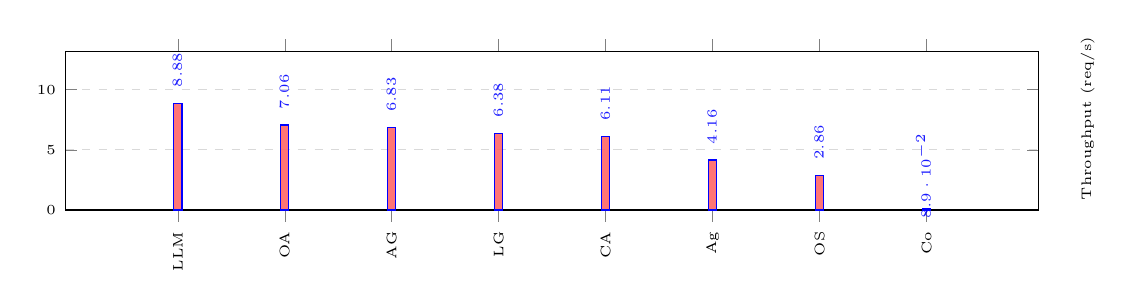
\begin{tikzpicture}
\begin{axis}[
    width=1.15\linewidth,
    height=3.6cm,
    ymin=0,
    ymax=13.206,
    % symbolic x coords={Direct LLM,OpenAgents,AutoGen,LangGraph,CrewAI,Agno,OpenAISDK,Concordia},
    symbolic x coords={ LLM,OA,AG,LG,CA,Ag,OS,Co},
    xtick=data,
    xticklabel style={rotate=90, anchor=east, font=\tiny},
    ylabel={Throughput (req/s)},
    ylabel style={at={(axis description cs:1.05,0.)}, anchor=west},
    tick label style={font=\tiny},
    ylabel style={font=\tiny},
    xlabel style={font=\tiny},
    ybar,
    bar width=3pt,
    enlarge x limits=0.15,
    ymajorgrids=true,
    grid style={dashed,gray!30},
    nodes near coords,
    nodes near coords style={
        font=\tiny,
        yshift=12pt,
        xshift=5pt,
        anchor=south,
        rotate=90
    },
    every axis plot/.append style={fill opacity=0.9},
]
% \addplot+[fill=red!60] coordinates {(Direct LLM,8.875) (OpenAgents,7.062) (AutoGen,6.827) (LangGraph,6.377) (CrewAI,6.113) (Agno,4.158) (OpenAISDK,2.860) (Concordia,0.089)};
\addplot+[fill=red!60] coordinates {(LLM,8.875) (OA,7.062) (AG,6.827) (LG,6.377) (CA,6.113) (Ag,4.158) (OS,2.860) (Co,0.089)};
\end{axis}
\end{tikzpicture}
\vspace{-3mm}
\caption{Throughput}
\end{subfigure}


\hspace{-2mm}
% ---------------- Mean Output ---------------- 
\begin{subfigure}{0.42\linewidth}
%\centering
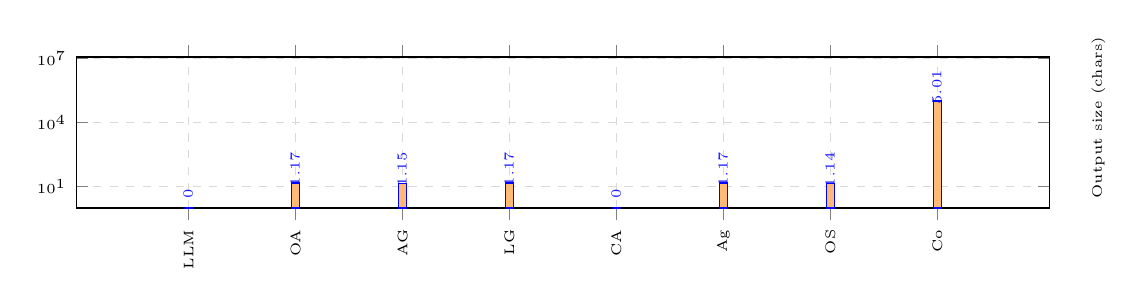
\begin{tikzpicture}
\begin{semilogyaxis}[
    width=1.15\linewidth,
    height=3.5cm,
    ymode=log,
    log basis y=10,
    ymin=1,
    ymax=11799100.564,
    % symbolic x coords={Direct LLM,OpenAgents,AutoGen,LangGraph,CrewAI,Agno,OpenAISDK,Concordia},
    symbolic x coords={ LLM,OA,AG,LG,CA,Ag,OS,Co},
    xtick=data,
    grid=major,
    xticklabel style={rotate=90, anchor=east, font=\tiny},
    ylabel={Output size (chars)},
    ylabel style={at={(axis description cs:1.05,0.)}, anchor=west},
    tick label style={font=\tiny},
    ymajorgrids=true,
    grid style=dashed,
    ylabel style={font=\tiny},
    xlabel style={font=\tiny},
    ybar,
    bar width=3pt,
    enlarge x limits=0.15,
    ymajorgrids=true,
    grid style={dashed,gray!30},
    nodes near coords,
    nodes near coords style={
        font=\tiny,
        yshift=5pt,
        xshift=5pt,
        anchor=south,
        rotate=90
    },
    every axis plot/.append style={fill opacity=0.9}
]
% \addplot+[fill=orange!60] coordinates {(Direct LLM,1.000) (OpenAgents,14.900) (AutoGen,14.220) (LangGraph,14.900) (CrewAI,1.000) (Agno,14.800) (OpenAISDK,13.880) (Concordia,102601.360)};
\addplot+[fill=orange!60] coordinates {
    (LLM,1.000) (OA,14.900) (AG,14.220) (LG,14.900)
    (CA,1.000) (Ag,14.800) (OS,13.880) (Co,102601.360)
};

\end{semilogyaxis}
\end{tikzpicture}
\vspace{-3mm}
\caption{Mean output}
\end{subfigure}
% ---------------- Output Summary ----------------
\hspace{-4mm} 
\begin{subfigure}{0.57\linewidth}
%\centering
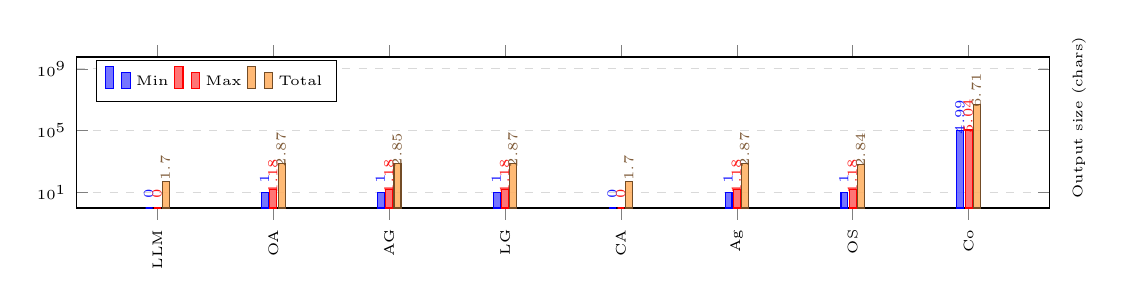
\begin{tikzpicture}
\begin{axis}[
    width=1.15\linewidth,
    height=3.5cm,
    ymode=log,
    log basis y=10,
    ymin=1,
    ymax=5899578000.200,
    % symbolic x coords={Direct LLM,OpenAgents,AutoGen,LangGraph,CrewAI,Agno,OpenAISDK,Concordia},
    symbolic x coords={ LLM,OA,AG,LG,CA,Ag,OS,Co},
    xtick=data,
    xticklabel style={rotate=90, anchor=east, font=\tiny},
    ylabel={Output size (chars)},
    ylabel style={at={(axis description cs:1.03,0.)}, anchor=west},
    legend style={
    at={(0.02,0.98)},
    anchor=north west,
    font=\tiny,
    legend columns=-1
    },
    tick label style={font=\tiny},
    ylabel style={font=\tiny},
    xlabel style={font=\tiny},
    ybar,
    bar width=2.5pt,
    enlarge x limits=0.1,
    ymajorgrids=true,
    grid style={dashed,gray!30},
    nodes near coords,
    nodes near coords style={
        font=\tiny,
        yshift=5pt,
        xshift=5pt,
        anchor=south,
        rotate=90
    },
    every axis plot/.append style={fill opacity=0.9}
]
% \addplot+[fill=blue!60] coordinates {(Direct LLM,1.000) (OpenAgents,10.000) (AutoGen,10.000) (LangGraph,10.000) (CrewAI,1.000) (Agno,10.000) (OpenAISDK,10.000) (Concordia,97448.000)};
% \addplot+[fill=red!60] coordinates {(Direct LLM,1.000) (OpenAgents,15.000) (AutoGen,15.000) (LangGraph,15.000) (CrewAI,1.000) (Agno,15.000) (OpenAISDK,15.000) (Concordia,110886.000)};
% \addplot+[fill=orange!60] coordinates {(Direct LLM,50.000) (OpenAgents,745.000) (AutoGen,711.000) (LangGraph,745.000) (CrewAI,50.000) (Agno,740.000) (OpenAISDK,694.000) (Concordia,5130068.000)};
\addplot+[fill=blue!60, bar shift=-3pt] coordinates {
    (LLM,1.000) (OA,10.000) (AG,10.000) (LG,10.000)
    (CA,1.000) (Ag,10.000) (OS,10.000) (Co,97448.000)
};

\addplot+[fill=red!60, bar shift=-0pt] coordinates {
    (LLM,1.000) (OA,15.000) (AG,15.000) (LG,15.000)
    (CA,1.000) (Ag,15.000) (OS,15.000) (Co,110886.000)
};

\addplot+[fill=orange!60, bar shift=3pt] coordinates {
    (LLM,50.000) (OA,745.000) (AG,711.000) (LG,745.000)
    (CA,50.000) (Ag,740.000) (OS,694.000) (Co,5130068.000)
};

\legend{Min, Max, Total}
\end{axis}
\end{tikzpicture}
\vspace{-7mm}
\caption{Output summary}
\end{subfigure}
\hfill
\vspace{0mm}
\noindent\fbox{%
  \parbox{0.85\linewidth}{\scriptsize
  \textbf{Abbreviations:}
  LLM=Direct LLM;
  OA=OpenAgents;
  AG=AutoGen;
  LG=LangGraph; \\
  CA=CrewAI;
  Ag=Agno;
  OS=OpenAI SDK;
  Co=Concordia.
  }
}
\vspace{-4mm}
\caption{
Framework overhead on a trivial task (“What is 2+2?”) over 50 trials.
Frameworks are ordered by p50 latency.
}
\vspace{-4mm}
\label{fig:framework-overhead}
\end{figure}





\noindent\textbf{Accuracy and Reasoning Effects.}
Accurate Retrieval (AR) measures factual recall and multi-hop reasoning over long contexts and is driven primarily by retrieval-based architectures rather than raw context accumulation. As shown in Table~\ref{tab:memorybench-results}, hybrid retrieval–accumulation performs best: LangGraph ($W{=}512$) achieves an average AR score of \emph{44.9}, exceeding pure retrieval (\emph{33.2}) and accumulation-based designs such as Agno (\emph{19.1}). Retrieval-centric designs remain robust on multi-hop and event-centric queries that require selective evidence access, while bounded accumulation provides limited gains via local coherence. Accumulation-only memory improves initially—peaking at \emph{32.3} for the OpenAI SDK at $W{=}1024$—but then degrades as unfiltered context dilutes relevance. Overall, reliable factual recall depends on architectural retrieval mechanisms, not larger context windows.
%
Long-Range Understanding (LRU), which evaluates cross-document abstraction and narrative reasoning, shows a similar pattern. Retrieval-first designs dominate, with retrieval-only LangGraph achieving the highest score (\emph{30.4}) through coherent summarization and multi-document reasoning. Accumulation-based designs approach this level only at very large context windows (OpenAI SDK at $W{=}8192$: \emph{27.5}), but with higher cost and instability. Hybrid designs perform worse on LRU as short-term accumulation interferes with retrieved narratives and weakens temporal coherence. These results indicate that exposing contiguous history instead of structured retrieval undermines robustness and efficiency.


\smallskip
\noindent\textbf{In-Session Learning and Knowledge Revision.}
Test-Time Learning (TTL), which evaluates in-session acquisition of concepts and preferences, shows the opposite trend. Accumulation-based designs improve steadily as interaction history grows, with the OpenAI SDK increasing from \emph{1.2} at $W{=}50$ to \emph{20.7} at $W{=}8192$. However, hybrid designs consistently outperform pure accumulation: LangGraph ($W{=}1024$) achieves the highest TTL score (\emph{28.9}) by anchoring learning to retrieved relevant signals rather than raw prompt growth. Retrieval-only memory performs poorly on TTL, confirming that adaptation requires accumulation but benefits from architectural filtering.
%
Selective Forgetting (SF), which probes controlled revision of outdated knowledge, remains largely unsupported across all frameworks. Retrieval-centric designs partially support single-hop forgetting, with retrieval-only LangGraph reaching an SF average of \emph{20.2}, but multi-hop forgetting remains below \emph{5.0} across all architectures (Table~\ref{tab:memorybench-results}). Accumulation-based designs perform worse even at large context sizes, and hybrid designs collapse as outdated information persists simultaneously in retrieval stores and accumulated context. This highlights the lack of explicit memory editing and dependency-aware deletion mechanisms in current frameworks.

\smallskip
\begin{figure}[t]
\centering
\vspace{2mm}
\setlength{\abovecaptionskip}{2pt}
\setlength{\belowcaptionskip}{-6pt}
\begin{tikzpicture}
\begin{groupplot}[
  group style={group size=2 by 1, horizontal sep=0.3cm},
  width=0.52\linewidth,
  height=0.38\linewidth,
  symbolic x coords={50,512,1024,2048,4096,8192},
  xtick=data,
  xlabel={Context Window (tokens)},
  ylabel={Total Runtime (s)},
  grid=both,
  grid style={dashed,gray!30},
  tick label style={font=\scriptsize},
  label style={font=\scriptsize},
  title style={font=\scriptsize, yshift=-7}, % ← THIS LINE
  legend style={
  font=\scriptsize,
  draw=none,
  legend image code/.code={
    \draw[mark size=0.8pt]
      plot coordinates {(0cm,0cm) (0.2cm,0cm)};
  }
}
]
% -------- Left: LangGraph --------
\nextgroupplot[
  yshift=10pt,
  title={LangGraph},
  legend style={at={($(0,0)+(-1cm,-1cm)$)},legend columns=1,fill=none,draw=black,anchor=center,align=center},
  legend to name=fred
]

\addplot+[mark=*, mark size=1.2pt, thick, blue]
  coordinates {(50,4236.5) (512,4538.9) (1024,4495.4) (2048,5093.6) (4096,5817.5) (8192,6705.5)};
\addlegendentry{AR}

\addplot+[mark=*, mark size=1.2pt, thick, orange]
  coordinates {(50,2247.6) (512,2336.1) (1024,2487.4) (2048,2607.0) (4096,2896.3) (8192,3323.9)};
\addlegendentry{TTL}

\addplot+[mark=*, mark size=1.2pt, thick, green!60!black]
  coordinates {(50,529.3) (512,523.5) (1024,507.1) (2048,548.7) (4096,531.4) (8192,541.3)};
\addlegendentry{LRU}

\addplot+[mark=*, mark size=1.2pt, thick, red]
  coordinates {(50,1861.8) (512,2043.3) (1024,2049.5) (2048,2094.1) (4096,2086.5) (8192,2099.3)};
\addlegendentry{SF}

% -------- Right: OpenAI SDK --------
\nextgroupplot[
  title={OpenAI SDK},
  ylabel={},
  yticklabels={},
  ytick=\empty,
]

\addplot+[mark=*, mark size=1.2pt, thick, blue]
  coordinates {(50,5475.7) (512,5192.0) (1024,4829.4) (2048,5266.9) (4096,5838.1) (8192,6955.1)};

\addplot+[mark=*, mark size=1.2pt, thick, orange]
  coordinates {(50,2175.9) (512,2557.4) (1024,3064.1) (2048,2807.4) (4096,2733.7) (8192,2873.4)};

\addplot+[mark=*, mark size=1.2pt, thick, green!60!black]
  coordinates {(50,1650.0) (512,1598.0) (1024,1479.2) (2048,1609.5) (4096,1805.3) (8192,2316.5)};

\addplot+[mark=*, mark size=1.2pt, thick, red]
  coordinates {(50,2450.6) (512,1846.7) (1024,1832.3) (2048,1978.4) (4096,1718.5) (8192,3382.1)};

\end{groupplot}
% {\pgfplotslegendfromname{fred}};
\node[
  anchor=west,
  xshift=6pt
] at (group c2r1.east) {\ref{fred}};
\end{tikzpicture}
\caption{Runtime as a function of context window for LangGraph (left) and OpenAI SDK (right) across the four task.}
\label{fig:runtime-vs-context}
\vspace{-4mm}
\end{figure}

\noindent\textbf{Runtime and Scalability Effects.}
Figure~\ref{fig:runtime-vs-context} reports runtime as a function of context window for LangGraph (hybrid retrieval–accumulation) and the OpenAI SDK (pure accumulation) across the four MemoryAgentBench competencies. Each task ingests shared context and issues multiple queries, so cost scales with both context size and query count. High-query tasks such as Accurate Retrieval and Test-Time Learning exhibit steep runtime growth under accumulation, where full histories are replayed for each query. In contrast, Long-Range Understanding remains nearly flat for LangGraph due to few queries per session, while Selective Forgetting shows moderate growth. Overall, accumulation drives rapid cost escalation as context grows, whereas retrieval avoids repeated processing. These results demonstrate that scalability is governed by memory architecture rather than by the LLM’s nominal context capacity.

\smallskip
\noindent\textbf{Summary.}
Memory behavior in multi-agent frameworks is governed by architecture, not context length alone. Retrieval enables stable recall and global reasoning, accumulation enables in-session learning but scales poorly, and hybrid designs are effective only under bounded context. The absence of explicit memory editing primitives prevents reliable knowledge revision, motivating future architectural support for safe and controllable long-term memory.



%